\subsection{Further prefix sum optimization}
Again we are interested in computing the prefix sum for some $f \in R^{\mZ}$,
\[
    \Sigma_{f}(n) \coloneqq\sum_{k = 1}^{n} f(k).
\]

 If we want to compute $\Sigma_{f}(n)$, then we will search a decomposition
$h = g*f$.

We start by giving two important lemmas.
\begin{lemma}\label{lem: division lemma}
    Let $k_1,k_2,k_3 \in \mZ$, then
    \[
        \left\lfloor \frac{\left\lfloor \frac{k_1}{k_2} \right\rfloor }{k_3} \right\rfloor = 
        \left\lfloor \frac{k_1}{k_2 \cdot k_3} \right\rfloor .
    \]
\end{lemma}
\begin{proof}
    By the division algorithm for positive integers, there exists unique $q_1,r_1 \in \NN$ with
    $r_1 < k_2$ such that $k_1 = k_2 q_1 + r_1$.
    $q_1$ coincides with $\left\lfloor \frac{k_1}{k_2} \right\rfloor$.
    
    Again by the division algorithm for positive integers, there exists unique $q_2,r_2 \in \NN$ with
    $r_2 < k_3$ such that $q_1 = k_3 q_2 + r_2$.
    Therefore, 
    $q_2 = \left\lfloor \frac{q_1}{k_3} \right\rfloor = \left\lfloor \frac{\left\lfloor \frac{k_1}{k_2} \right\rfloor}{k_3}\right\rfloor$.
    
    Substituting $q_1 = k_3 q_2 + r_2$ in the first division yields that 
    \[
    k_1 = (k_2 k_3) q_2 + (k_2 r_2 + r_1).
    \]

    Next we prove that the previous equation is the integer division of $k_1$ by $k_2 k_3$. Since integer division is unique, we only need to check that $q_2, (k_2 r_2 + r_1) \in \NN$ and
    $k_2 r_2 + r_1 < k_2 k_3$. The first condition is obviously true and for the second one
    \[
    k_2 r_2 + r_1 < k_2r_2 + k_2 = k_2 (r_2 + 1) \leq k_2 k_3.
    \]

    By the uniqueness of integer division, 
    \[
    \left\lfloor \frac{\left\lfloor \frac{k_1}{k_2} \right\rfloor}{k_3}\right\rfloor = q_2 = \left\lfloor \frac{k_1}{k_2 k_3} \right\rfloor.
    \]
\end{proof}

\begin{lemma}\label{lemma: harmonic}
    Let $n \in \mZ$. Then
        \[
        \Card\left(\left\{ \left\lfloor \frac{n}{d}\right\rfloor \, \middle| \,  1 \leq d \leq n\right\}\right) \leq 2 \lfloor \sqrt{n} \rfloor.
        \]
\end{lemma}
\begin{proof}
         \[
        \Card\left(\left\{ \left\lfloor \frac{n}{d}\right\rfloor \, \middle| \,  1 \leq d \leq  \lfloor \sqrt{n} \rfloor\right\}\right) \leq \lfloor \sqrt{n} \rfloor.
        \]

        For every $d \in \{ \lfloor \sqrt{n} \rfloor +1,\dots, n\}$,
        $ 1 \leq \left\lfloor \frac{n}{d}\right\rfloor \leq \lfloor \sqrt{n} \rfloor$ since $0 = \left\lfloor \frac{n}{d \cdot(\lfloor \sqrt{n} \rfloor +1)}\right\rfloor
        =\left\lfloor \frac{\left\lfloor \frac{n}{d}\right\rfloor}{\lfloor \sqrt{n} \rfloor +1} \right\rfloor $. Therefore, 
                \[
                \begin{aligned}
        \Card &\left(\left\{ \left\lfloor \frac{n}{d}\right\rfloor \, \middle| \,   1 \leq d \leq n \right\}\right) = \\
           &\Card\left(\left\{ \left\lfloor \frac{n}{d}\right\rfloor \, \middle| \,  1 \leq d \leq \lfloor \sqrt{n} \rfloor\right\}\right) +
              \Card\left(\left\{ \left\lfloor \frac{n}{d}\right\rfloor \, \middle| \,  \lfloor \sqrt{n} \rfloor+1 \leq d \leq n\right\}\right)
        \leq 2 \lfloor \sqrt{n} \rfloor.
                        \end{aligned}
        \]

\end{proof}

Now we begin with the optimization.
We suppose that $f \in R^{\mZ}$ can be decomposed as $h = f*g$, so more sophisticated techniques can be used to exploit the 
structure of \(f\). Then it is satisfied that
\[
\begin{aligned}
    \Sigma_{h}(n) &=\sum_{k = 1}^{n} h(k) =
   \sum_{k = 1}^{n} \sum_{d \mid k} g(d) \cdot f\left( \frac{k}{d}\right) = \\ &
   \sum_{d = 1}^{n} 
    \sum_{r = 1}^{\left\lfloor \frac{n}{d}  \right\rfloor} g(d) \cdot f(r) =
   \sum_{d = 1}^{n} g(d) \cdot
   \left( \sum_{r = 1}^{\left\lfloor \frac{n}{d}  \right\rfloor} f(r)\right) = \sum_{d = 1}^{n} g(d) \cdot \Sigma_{f}\left( \left\lfloor \frac{n}{d}  \right\rfloor \right).
\end{aligned}
\]

We can isolate the term for $d = 1$, which gives us 
\[
\begin{aligned}
    \Sigma_{h}(n) &= g(1) \cdot \Sigma_{f}\left( 
   n \right) +\sum_{d = 2}^{n} g(d) \cdot \Sigma_{f}\left( \left\lfloor \frac{n}{d}  \right\rfloor \right).
\end{aligned}
\]

If $g(1) \neq 1$ and we can solve for $\Sigma_{f}$, which yields
\[
    \Sigma_{f}(n) = \frac{\Sigma_{h}(n) - \sum_{d = 2}^{n} g(d) \cdot \Sigma_{f}\left( \left\lfloor \frac{n}{d}  \right\rfloor \right)}{g(1)}.
\]

Let 
\begin{gather*}
      A^{-}(n) \coloneqq \left\{ \left\lfloor \frac{n}{d}\right\rfloor \, \middle| \,  1 \leq d \leq  \lfloor \sqrt{n} \rfloor\right\}, \\
         A^{+}(n) \coloneqq \left\{ \left\lfloor \frac{n}{d}\right\rfloor \, \middle| \,   \lfloor \sqrt{n} \rfloor+ 1 \leq d \leq n\right\},\\
         A(n) \coloneqq A^{-}(n) \sqcup A^{+}(n).
\end{gather*}

As we have seen in Lemma \ref{lemma: harmonic}, the elements of
$A^{+}(n)$ are bounded above by $\lfloor \sqrt{n} \rfloor$ while the elements of $A^{-}(n)$ are bounded bellow by $\lfloor \sqrt{n} \rfloor$, since the sequence $\left\lfloor \frac{n}{1} \right\rfloor, \left\lfloor \frac{n}{3} \right\rfloor,\dots, \left\lfloor \frac{n}{n} \right\rfloor$ is non-increasing and
$\lfloor \sqrt{n} \rfloor^{2} \leq n$.
There are a lot more indices in $A^{+}(n)$ than in $A^{-}(n)$, but
in  $A^{+}(n)$ several indices collapse to the same value.

Since the sequence $\left\lfloor \frac{n}{1} \right\rfloor, \left\lfloor \frac{n}{3} \right\rfloor,\dots, \left\lfloor \frac{n}{n} \right\rfloor$ is non-increasing, we can compute an interval partition of $\{1,\dots,n\}$ such that each interval represents
a value of the sequence. Suppose we have $d \in \{1,\dots,n\}$, 
how can we compute the interval that contains $d$?

Let $\left \lfloor \frac{n}{d} \right\rfloor = k$, then for every element $x$ of the same interval as $d$ is satisfied that
\[
 k \leq \frac{n}{x} < k+1.
\]

Solving for $x$ we get that $\left \lfloor \frac{n}{x} \right\rfloor = k$ if and only if
\[
\frac{n}{k+1} < x \leq \frac{n}{k}.
\]
That last condition can be written as
$x \in \left\{ \left\lfloor \frac{n}{k+1} \right\rfloor + 1, \dots,
 \left\lfloor \frac{n}{k} \right\rfloor \right\}$, so the interval of
 $d$ is 
 \[\left\{ \left\lfloor \frac{n}{\left \lfloor \frac{n}{d} \right\rfloor+1} \right\rfloor + 1, \dots,
 \left\lfloor \frac{n}{\left \lfloor \frac{n}{d} \right\rfloor} \right\rfloor \right\}.\]

 This characterization and the Lemma \ref{lemma: harmonic} gives us an algorithm in $\cO(\sqrt{n})$ that computes iteratively the desired interval partition. Let $\overline{A}$ be such partition. The formula for the prefix sum becomes
 \[
    \Sigma_{f}(n) = \frac{\Sigma_{h}(n) - \sum_{(a,b) \in \overline{A}}  \left( \Sigma_{g}(b) - \Sigma_{g}(a-1)\right)\cdot \Sigma_{f}\left( \left\lfloor \frac{n}{a}  \right\rfloor \right)}{g(1)}.
\]

At first it may seem that this formula is recursive but
Lemma \ref{lem: division lemma} assures us we only need to compute the values that belongs to $A(n)$ in all the recursive calls of the function. Therefore, this can be put as a triangular linear system of
$\cO(\sqrt{n})$ variables and equations that can be solved via substitution. It is important to notice that the equation with value
$\left\lfloor \frac{n}{d} \right\rfloor$ associated involves at most
$ 2 \cdot \sqrt{\left\lfloor \frac{n}{d} \right\rfloor}$ terms by Lemma \ref{lemma: harmonic}.
We suppose that we can compute $\Sigma_{g}(k)$  in $\cO(1)$ and $\Sigma_{h}(k)$  in $\cO(\sqrt{k})$.

In conclusion, the cost for solving the variables belonging to 
$A^{+}(n)$ is in $\cO\left(\sum_{i = 1}^{\lfloor \sqrt{n} \rfloor}\sqrt{i}\right)$, where it is included the cost for computing $\Sigma_{h}$.

In order to better understand the cost, we prove the following lemma
\begin{lemma}\label{lem: sum  cost}
Let $\alpha \in [0,1]$. For every $k \in \mZ$,
    \[
    \sum_{i = 1}^{k} i^{\alpha} \leq k^{1+\alpha}.
    \]
    In particular, $\cO(\sum_{i = 1}^{k} i^{\alpha}) \subseteq 
    \cO(k^{1+\alpha})$.
\end{lemma}
\begin{proof}
    
We will show it by induction on $k$.
It is obviously true for $k = 1$ and if it is satisfied by $k$,
then 
\[
	  \sum_{i = 1}^{k+1} i^{\alpha} =
    \sum_{i = 1}^{k} i^{\alpha}+ (k+1)^{\alpha} \leq  k^{\alpha + 1} + (k+1)^{\alpha}.
\]
Dividing by $(k+1)^{\alpha}$ the last equation, we obtain that
\[
	 \frac{\sum_{i = 1}^{k+1} i^{\alpha}}{(k+1)^{\alpha}}  \leq  \frac{k^{\alpha + 1}}{(k+1)^{\alpha}} + \frac{(k+1)^{\alpha}}{(k+1)^{\alpha}} = 
	 k \cdot \left(\frac{k}{k+1}\right)^{\alpha} +1 \leq k \cdot 1 + 1 = (k+1) .
\]

Multiplying  both sides by 
$(k+1)^{\alpha}$ gives the wanted result to prove the induction hypothesis
\[
	 \sum_{i = 1}^{k+1} i^{\alpha} \leq  (k+1)^{1+\alpha} .
\]

\end{proof}

Therefore,
\[
    \sum_{i = 1}^{\lfloor \sqrt{n} \rfloor} \sqrt{i} \leq 
    \lfloor \sqrt{n} \rfloor^{\frac{3}{2}} \leq 
     \left(\sqrt{n}\right)^{\frac{3}{2}} = n^{\frac{3}{4}}.
\]



We deduce that the cost for solving the variables belonging to 
$A^{+}(n)$ is in $\cO(n^{\frac{3}{4}})$.

Now, for solving the variables of $A^{-}(n)$, the cost is given by
$\cO\left( \sum_{i = 1}^{\lfloor \sqrt{n} \rfloor} \sqrt{\left\lfloor \frac{n}{i} \right\rfloor} \right) = 
\cO\left( \sum_{i = 1}^{\lfloor \sqrt{n} \rfloor} \frac{\sqrt{n} }{\sqrt{i}} \right) = \cO\left( \sum_{i = 1}^{\lfloor \sqrt{n} \rfloor} \frac{\lfloor \sqrt{n} \rfloor}{\sqrt{i}} \right)$, where it is included the cost for computing $\Sigma_{h}$.

As before, in order to better understand the cost, we prove 
a lemma.

\begin{lemma}\label{lem: sum inv cost} Let $\alpha \in [0,1)$.
    For every $k \in\mZ $,
    \[
    \frac{(k+1)^{1-\alpha}-1}{1-\alpha} \leq 
    \sum_{i = 1}^{k} \frac{1}{i^{\alpha}} \leq \frac{k^{1-\alpha}-\alpha}{1-\alpha}.
    \]
        In particular, $\cO(\sum_{i = 1}^{k} i^{-\alpha}) = 
    \cO(k^{1-\alpha})$.
\end{lemma}
\begin{proof}

Let $f: [1, +\infty) \rightarrow \RR$ be defined as $f(x) = x^{-\alpha}$, 
$g: [1, +\infty) \rightarrow \RR$  as 
$f(x) = \lfloor x \rfloor^{-\alpha}$, and
$h: [1, +\infty) \rightarrow \RR$ as
\begin{equation*}
h(x) = 
\begin{cases}
1, & \text{if } x \in [1,2).\\[2mm]
f(x-1), & \text{if } x \in [2,\infty).
\end{cases}
\end{equation*}

The following diagram that shows $f$, $g$, and $h$ for $\alpha = 0.4$.

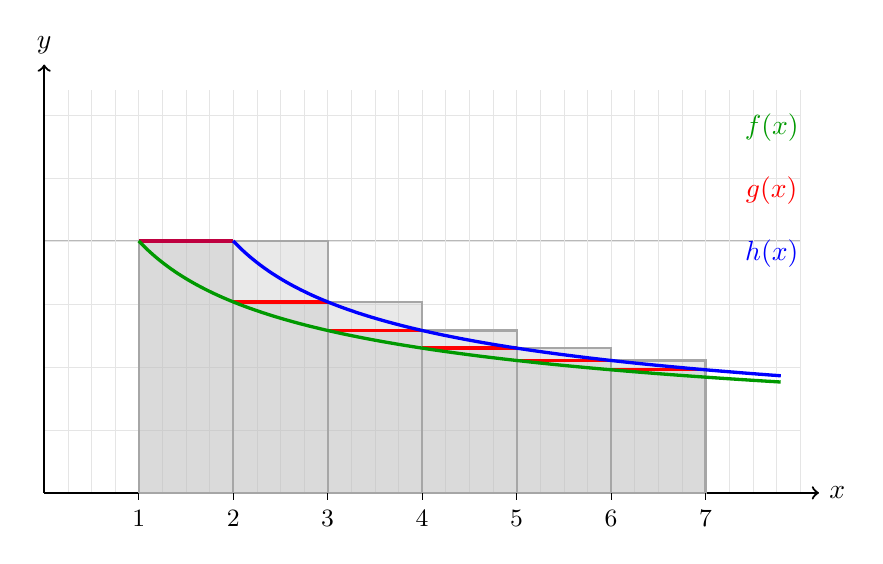
\begin{tikzpicture}[
  x=1.2cm,
  y=3.2cm
]
\def\alpha{0.4}

%--------------------
% Rejilla
%--------------------
\draw[step=1, gray!55, thin] (0,0) grid (8,1.6);
\draw[step=0.25, gray!20, very thin] (0,0) grid (8,1.6);

%--------------------
% Ejes
%--------------------
\draw[->, thick] (0,0) -- (8.2,0) node[right] {$x$};
\draw[->, thick] (0,0) -- (0,1.7) node[above] {$y$};

%--------------------
% Rectángulos (cajas) — gris semitransparente
%--------------------
\foreach \i in {1,...,6} {
  \filldraw[
    fill=gray!50,
    fill opacity=0.35,
    draw=gray!70,
    thick
  ]
  (\i,0) rectangle (\i+1, {(\i)^(-\alpha)});
}

% h(x)=1 en [1,2)
\filldraw[
  fill=gray!50,
  fill opacity=0.35,
  draw=gray!70,
  thick
] (1,0) rectangle (2,1);

% h(x)=f(x-1) para x>=2
\foreach \i in {2,...,6} {
  \filldraw[
    fill=gray!50,
    fill opacity=0.35,
    draw=gray!70,
    thick
  ]
  (\i,0) rectangle (\i+1, {(\i-1)^(-\alpha)});
}

%--------------------
% g(x) escalonada
% Primer tramo morado, el resto rojo, sin desplazamiento
%--------------------
\draw[very thick, purple] (1,1) -- (2,1); % primer tramo

\foreach \i in {2,...,6} {
  \draw[very thick, red] (\i, {(\i)^(-\alpha)}) -- (\i+1, {(\i)^(-\alpha)});

}

%--------------------
% Curva f(x) — verde (por encima)
%--------------------
\draw[
  very thick,
  green!60!black,
  domain=1:7.8,
  samples=400
] plot (\x, {\x^(-\alpha)});

%--------------------
% Curva h(x) — azul (por encima)
%--------------------
\draw[
  very thick,
  blue,
  domain=2:7.8,
  samples=400
] plot (\x, {(\x-1)^(-\alpha)});

%--------------------
% Etiquetas arriba a la derecha
%--------------------
\node[green!60!black] at (7.7,1.45) {$f(x)$};
\node[red] at (7.7,1.2) {$g(x)$};
\node[blue] at (7.7,0.95) {$h(x)$};

%--------------------
% Marcas eje x
%--------------------
\foreach \k in {1,...,7} {
  \draw (\k,0) -- (\k,-0.03) node[below] {\small $\k$};
}

\end{tikzpicture}

Since $f$ is monotonously decreasing, we have that
$f(x) \leq g(x) \leq h(x)$ for every $x \in [1,+\infty)$.

Furthermore, for $k \in \mZ$ it is satisfied that
\[
 \int_{1}^{k+1} g(x) \, dx = \sum_{i = 1}^{k} i^{-\alpha}.
 \]
 
 We can conclude that 
 \[
 \frac{(k+1)^{1-\alpha}-1}{1-\alpha} = 
 \int_{1}^{k+1} f(x) \, dx
 \leq  \int_{1}^{k+1} g(x) \, dx \leq 
 \int_{1}^{k+1} h(x) \, dx = 1 + \int_{1}^{k} f(x) \, dx
 = \frac{k^{1-\alpha}-\alpha}{1-\alpha}.
 \]



    
\end{proof}


Using last lemma with $k = \lfloor \sqrt{n} \rfloor$
proves that solving the variables in $A^{-}(n)$ can be done in
$\cO\left( \sum_{i = 1}^{\lfloor \sqrt{n} \rfloor} \frac{\lfloor \sqrt{n} \rfloor}{\sqrt{i}} \right) = \cO\left(n^{\frac{3}{4}} \right)$.

In conclusion, the whole algorithm runs in $\cO(n^{\frac{3}{4}})$.



Nevertheless, if $f$ is multiplicative we can precompute the values of $\Sigma_{f}$ in the range $\{1,\dots,m\}$ in $\cO(m)$ with a sieve.
Since we already have a cost in $\Omega(\sqrt{n})$ by iterating over the interval partition, we can suppose that $\lfloor \sqrt{n} \rfloor < m$. Therefore, our total cost would be in $\cO(m)$ for precomputing $\Sigma_{f}$ with a sieve and then
$\cO\left( \sum_{i = 1}^{\left\lfloor \frac{n}{m} \right\rfloor} \sqrt{\left\lfloor \frac{n}{i} \right\rfloor} \right) = \cO\left( \sqrt{n} \cdot \sum_{i = 1}^{\left\lfloor \frac{n}{m} \right\rfloor} \sqrt{\frac{ 1}{i}} \right) = \cO\left(\sqrt{n} \cdot \sum_{i = 1}^{\left\lfloor \frac{n}{m} \right\rfloor} \frac{ 1}{\sqrt{i}}
 \right) =
\cO\left( \frac{n}{\sqrt{m}} \right)$ for solving the remaining values of $\Sigma_{f}$ in $A^{-}(n)$.
Taking $\alpha \in [0,1]$ and $m = n^{\alpha}$ yields the total cost of
$\cO\left(\max\left\{ n^{\alpha}, n^{1 -\frac{\alpha}{2}}\right\}\right)$, which is minimized with
$\alpha = \frac{2}{3}$. 

The conclusion is that computing the prefix sum of such a multiplicative function can be done in $\cO\left(n^{\frac{2}{3}}\right)$ precomputing with a sieve $\Sigma_{f}$ until $\left\lfloor n^{\frac{2}{3}} \right\rfloor$ and then applying the previous algorithm. This method uses $\cO\left(n^{\frac{2}{3}}\right)$ extra space and can be further optimized with a segmented sieve reaching $\cO\left(\sqrt{n}\right)$ in extra space and $\tilde{\cO}(n^{\frac{2}{3}})$ time.

  



\newpage
\subsection*{Problems}

\newpage